\documentclass[handout]{beamer} % [handout] para imprimir eliminando transiciones

%\usefonttheme[onlymath]{serif}
%\usepackage{fontspec}
%\defaultfontfeatures{Mapping=tex-text}
%\setsansfont[Ligatures={Common}]{Futura}
%\setmonofont[Scale=0.8]{Monaco}

\usepackage{beamerthemesplit}
\usepackage[utf8]{inputenc}
\usepackage[spanish]{babel}
\mode<presentation>
\usetheme{default}
\usecolortheme{dolphin}
\usepackage{alltt}    % \begin{alltt}
\usepackage{amssymb}  % mathematical symbols
\usepackage{comment}
\usepackage{multicol} % \multicols
\usepackage{tabto}    % \tabto
\usepackage{verbatim} % comentarios

\title{Estructuras de datos}   %[titulo corto]
\author{Fabián Riquelme Csori} %[nombre corto]
\date{2017}                    %[fecha corta]
\institute{Universidad de Valparaíso}                 %[instituto corto]

\newcommand{\HRule}{\rule{\linewidth}{0.2mm}\\[1ex]}
\newcommand{\blue}[1]{\textcolor{blue}{#1}}
\newcommand{\red}[1]{\textcolor{red}{#1}}
\newcommand{\redb}[1]{{\color{red!70!black}{#1}}}
\newcommand{\green}[1]{{\color{green!70!black}{#1}}}
\newcommand{\gray}[1]{{\color{gray!50!white}{#1}}}
\newcommand{\textgreek}[1]{\begingroup\fontencoding{LGR}\selectfont#1\endgroup}
% \alert{texto destacado en rojo}
% \color{green} Color en verde
% \structure{texto en lila}

\begin{document}


%\begin{frame}%[plain]
%  \titlepage
%\end{frame}
%
% [opciones]:
% plain: oculta barra de navegacion, deja + espacio para contenido
% fragile: usar comandos como verbatim
% b,c,t: alineacion vertical
% label=nombre_etiqueta
% allowframebreaks: divide contenido en varios frames si es demasiado largo
% shrink: para escribir mucho texto en una transparencia, reduciendo tamano de fuente

%%%%%%%%%% PORTADA %%%%%%%%%%
\begin{frame}[plain]
  \begin{figure}[h]
    \begin{minipage}{0.3\textwidth}
    
\includegraphics[width=.9\textwidth]{./image/logo-UV.png}
    \end{minipage}
    \begin{minipage}{0.65\textwidth}
     $~$\\[3.6ex]
     \footnotesize{Escuela de Ingeniería Civil Informática}\\
     \footnotesize{Facultad de Ingeniería}
    \end{minipage}
  \end{figure}
  \begin{center}
    \vspace{1ex}
    \HRule
    \Large{Estructuras de datos}\\{\small Capítulo III: Árboles}\\[-1ex]
    \HRule\vspace{1ex}
    \large{Fabián Riquelme Csori}\\[.5ex]\footnotesize{fabian.riquelme@uv.cl}\\[6ex] {\tiny 2017-II}\\[6ex]
  \end{center}
\end{frame}

%%%%%%%%%% INDEX %%%%%%%%%%
\begin{frame}
 \frametitle{Index}
 \scriptsize 			% reducir tamano de letra
 \tableofcontents		%[pausesections]
\end{frame}

%%%%%%%%%%% ACTUAL INDEX %%%%%%%%%%
%\AtBeginSection[] %generar indice automaticamente
%{
%\begin{frame}<beamer>%[plain]
% \frametitle{Index}
% \framesubtitle{subtitulo}
% \scriptsize
% \tableofcontents[currentsection, currentsubsection]
%\end{frame}
%}

%==============================
\section{Árboles}

%-----------------------
\subsection{Fundamentos}

\begin{frame}{Definición general}
    \begin{itemize}
        \item<1-> Un \blue{grafo} es un par $G=(V,E)$ donde $V$ es un conjunto de nodos y $E$ un conjunto de aristas.
        \item<2-> Un \blue{árbol} es un grafo \redb{conexo}, \redb{acíclico} y \redb{no dirigido} (aunque se puede dibujar con aristas ``hacia abajo'').
    \end{itemize}
    \uncover<3>{
    \begin{center}
        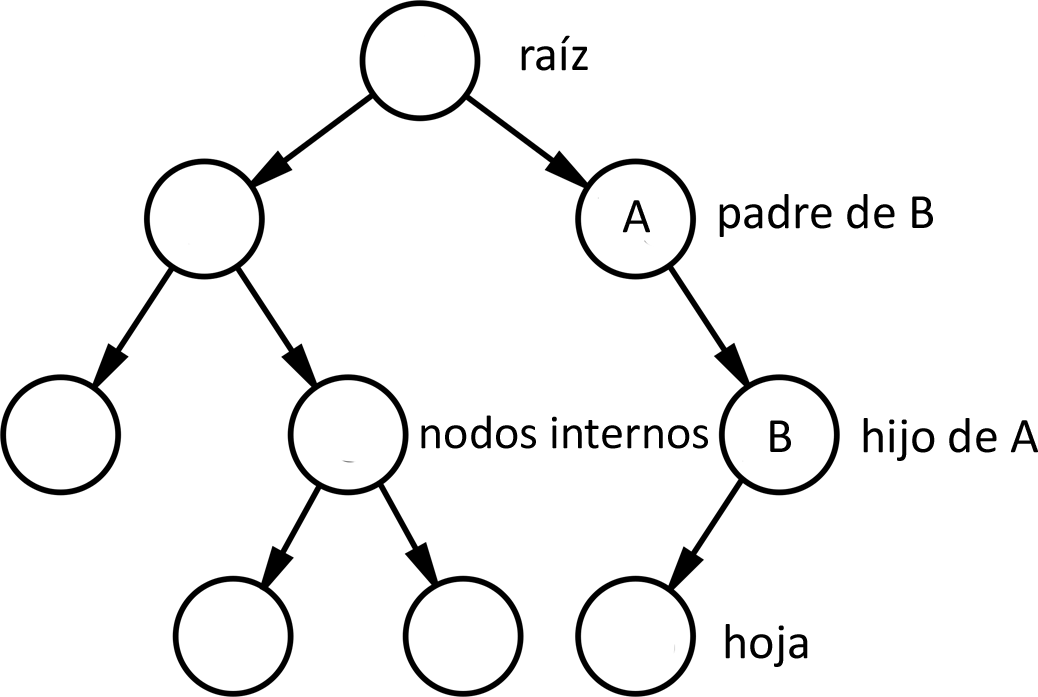
\includegraphics[width=.6\textwidth]{./image/cap3/tree1}
    \end{center}}
\end{frame}

\begin{frame}{Conceptos básicos}
    \begin{minipage}{0.6\textwidth}
    \begin{itemize}
        \item<1-> \textbf{Descendientes} de B: \blue{\{B,D,E,G,H\}}\\
        \uncover<2->{(conforman un \textbf{subárbol})}
        \item<3-> \textbf{Ascendientes} de F: \red{\{A,C,F\}}
        \item<4-> El \textbf{camino} A-H (secuencia de nodos A-B-E-H) tiene \textbf{largo} 3.
    \end{itemize}
    \end{minipage}
    \begin{minipage}{0.38\textwidth}
        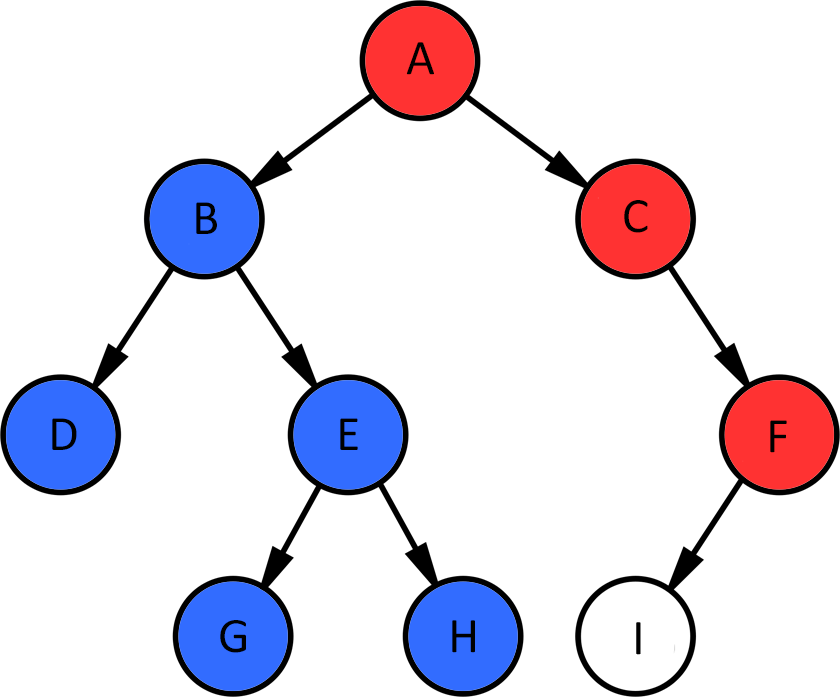
\includegraphics[width=\textwidth]{./image/cap3/tree2}
    \end{minipage}
\end{frame}

\begin{frame}{Conceptos básicos}
    \begin{center}
        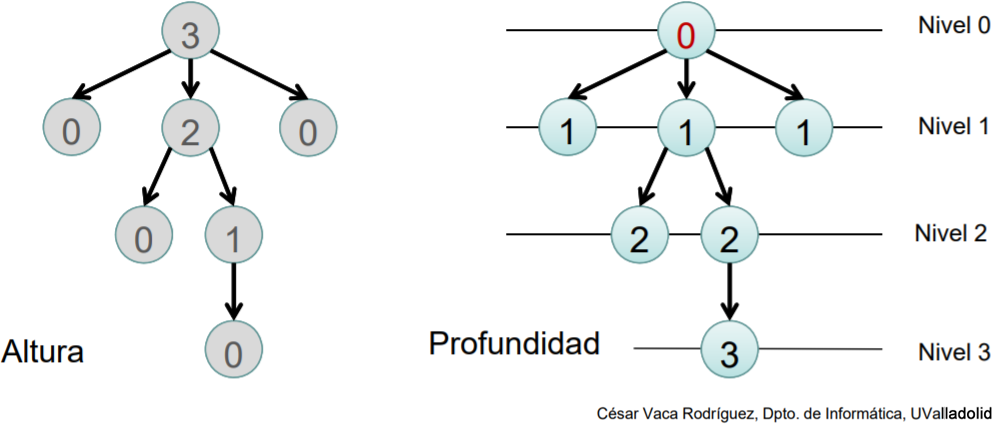
\includegraphics[width=\textwidth]{./image/cap3/tree3}
    \end{center}
    {\small
    \begin{itemize}
        \item<2-> ¿Cuál es la altura de una hoja? ¿del árbol? ¿de un nodo interno?
        \item<2-> ¿Cuál es la profundidad de la raíz? ¿de un nodo interno?
    \end{itemize}}
\end{frame}

\begin{frame}{Las aplicaciones son muchísimas...}
    \begin{minipage}{0.43\textwidth}
    \begin{center}
        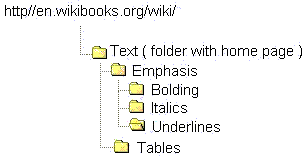
\includegraphics[width=\textwidth]{./image/cap3/folders-tree}
    \end{center}
    {\scriptsize Sistema de organización de carpetas.}
    \end{minipage}
    \begin{minipage}{0.55\textwidth}
    \begin{center}
        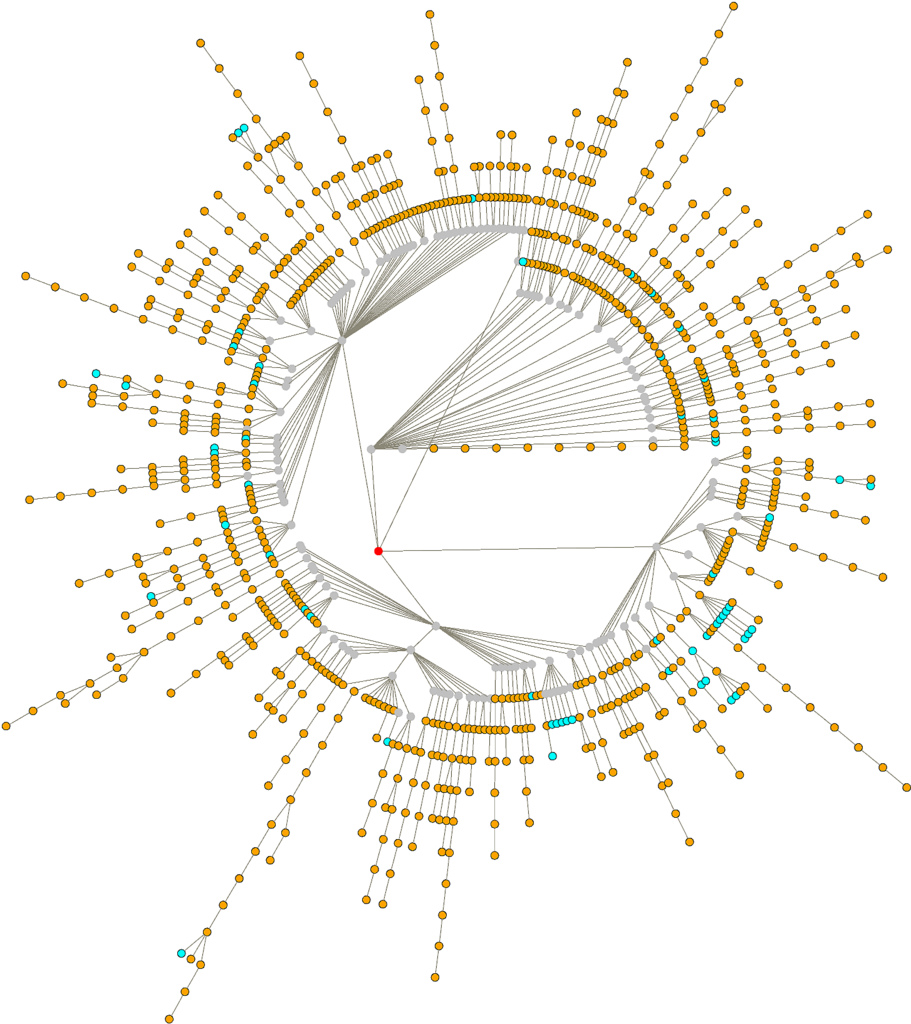
\includegraphics[width=.9\textwidth]{./image/cap3/Obama-tree.jpg}\\
    {\tiny Discusión {\em en:Presidency of Barack Obama}, Wikipedia.}
    \end{center}
    \end{minipage}
\end{frame}

%-----------------------
\subsection{Recorrido de árboles}

\begin{frame}{Recorrido de árboles}
    {\footnotesize
    \begin{itemize}
        \item \blue{Búsqueda en profundidad} o \blue{Depth-first search} (recursiva)
        \item \blue{Búsqueda en anchura} o \blue{Breadth-first search} (iterativa)
    \end{itemize}
    \begin{center}
        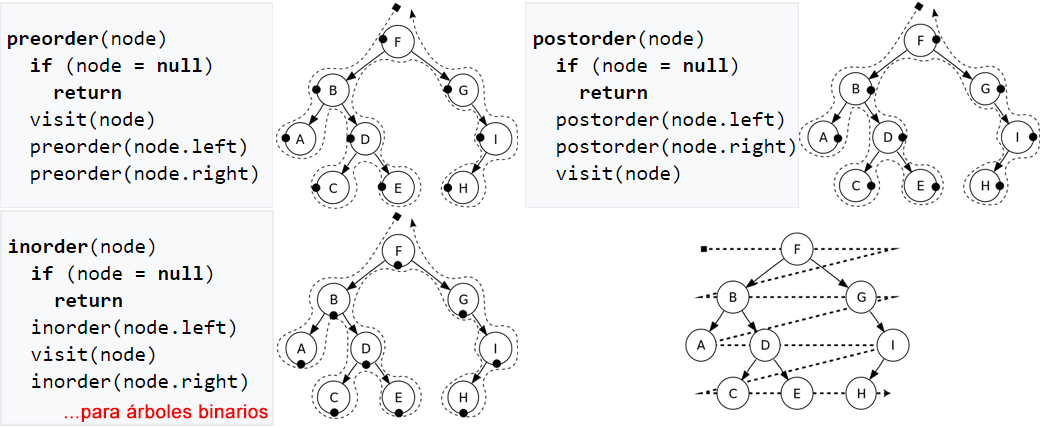
\includegraphics[width=\textwidth]{./image/cap3/recorrer-arbol}\\
    \end{center}}
\end{frame}

\begin{frame}{Ejemplo: Árboles sintácticos}
    \begin{minipage}{0.6\textwidth}
    \begin{itemize}
        \item Preorden (notación prefija):\\ * 1 + \^{} 3 4 2
        \item Postorden (notación postfija):\\
        1 3 4 \^{} 2 + *
        \item Inorden (notación habitual):\\
         1 * ((3 \^{} 4) + 2)
    \end{itemize}
    \end{minipage}
    \begin{minipage}{0.38\textwidth}
        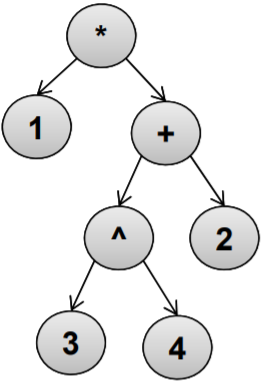
\includegraphics[width=.7\textwidth]{./image/cap3/tree-operations}
    \end{minipage}
\end{frame}

%------------------------------
\subsection{Árboles binarios}

\begin{frame}{Definiciones}

    {\small
    \begin{itemize}
        \item Un \blue{árbol binario} es un árbol donde cada nodo puede a lo más tener un hijo \redb{izquierdo} y un hijo \redb{derecho}.
        \item Es una estructura de datos (como lo era una lista enlazada).
    \end{itemize}}
    \begin{center}
        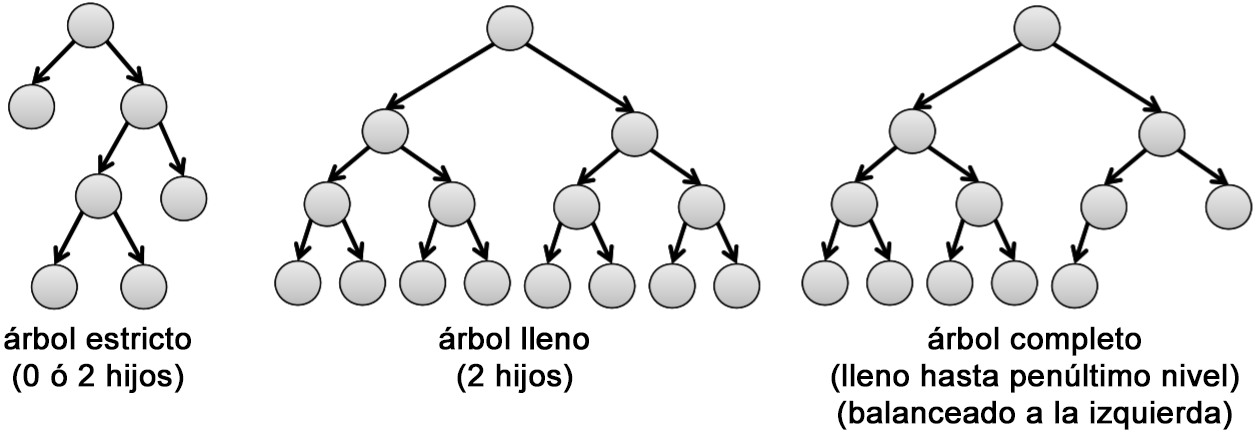
\includegraphics[width=\textwidth]{./image/cap3/arboles-binarios}
    \end{center}
    \pause
    {\small ¿Cuántos nodos tiene un árbol estricto en función de su altura $h$?}
\end{frame}

\begin{frame}{Árboles completos}
    \begin{itemize}
        \item<1-> En árboles completos, $h\in O(\log n)$
        \item<2-> Un árbol completo puede almacenarse en un \blue{vector} dado por sus orden \redb{recorrido por niveles}, de modo que para el \blue{índice} de cada nodo podemos conocer su \redb{padre} y sus \redb{hijos}.
    \end{itemize}
    \uncover<2->{
    \begin{center}
        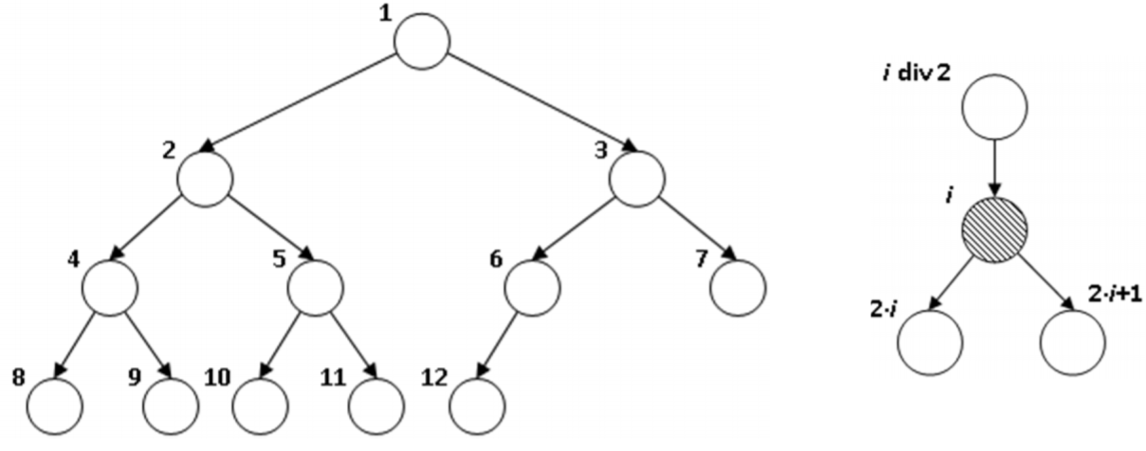
\includegraphics[width=.9\textwidth]{./image/cap3/completos}
    \end{center}}
\end{frame}

\begin{frame}{Ejercicio}
    \begin{enumerate}
        \item Ingrese aquí:\\
        \blue{\tiny \url{https://sites.google.com/site/programacioniiuno/temario/unidad-5---grafos/rboles}}
        \item Inspeccione el código descrito, también descargable aquí:\\
        \blue{\tiny \url{https://xp-dev.com/svn/uqbar/examples/prog2/unidad5-recursividadYArboles/arboles/}}
        \item ¿Cuál es la estructura de datos usada para manipular árboles?
        \item Testee las funciones \texttt{agregarElemento}, \texttt{buscarSubarbol}, \texttt{profundidad} y \texttt{grado}. ¿Qué es el \blue{grado} en este código?
        \item Testee los mecanismos de recorrido del árbol, en profundidad y en anchura. ¿Qué tipo de recorrido en profundidad se ha implementado? ¿preorder, inorder o postorder?
        \item Modifique el código para recorrer el árbol con los dos mecanismos de profundidad restantes. \green{(+5 pts)}
    \end{enumerate}
\end{frame}

%==============================
\section{Árboles balanceados}

%------------------------------
\subsection{Montículos (Heaps)}

\begin{frame}{Montículos (Heaps)}
    Un \blue{montículo} (\blue{heap}) es un \redb{árbol completo} tal que el valor de cada nodo es $\leq$ que el de sus \redb{descendientes} {\small ($\leq$ puede reemplazarse por $\geq$)}.
    \begin{center}
        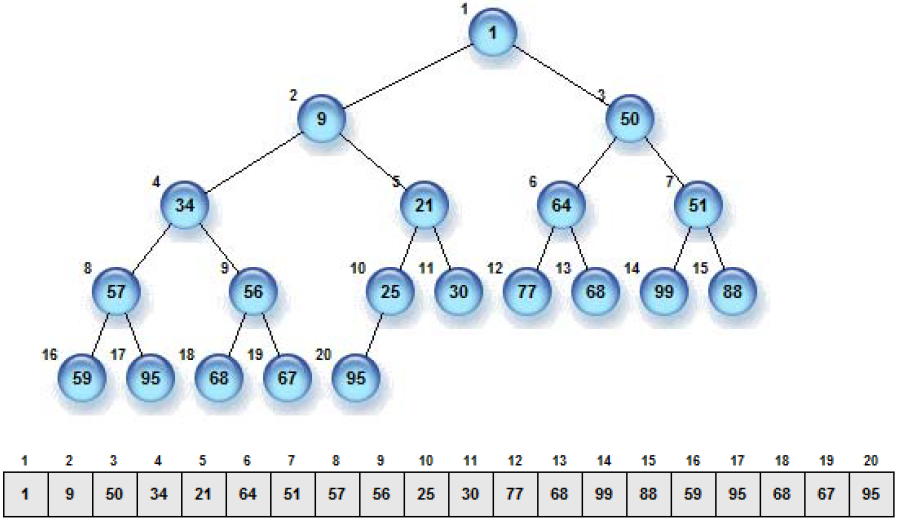
\includegraphics[width=.9\textwidth]{./image/cap3/heap}
    \end{center}
\end{frame}

\begin{frame}{Propiedades de un montículo}

    {\footnotesize
    \begin{itemize}
        \item<1-> El valor de la raíz es el mínimo.
        \item<2-> Sea $h$ la altura y $n$ el número de nodos, entonces $h\in O(\log n)$\\
        (son árboles completos).
        \item<3-> Si solo un nodo está mal ubicado, puede corregirse en $O(h)$.
    \end{itemize}}
    \uncover<4->{
    \begin{block}{Operaciones fundamentales}
    {\footnotesize
        \begin{itemize}
            \item<4-> \blue{Inserción}
            \begin{enumerate}
              \item El nuevo nodo se ubica al final del vector.
              \item Se {\em asciende} hasta que quede bien ubicado según su valor.
            \end{enumerate}
            \item<5-> \blue{Eliminar la raíz}
            \begin{enumerate}
              \item Se intercambia con la última hoja.
              \item Se desciende la nueva raíz hasta que quede bien ubicada según su valor.
            \end{enumerate}
        \end{itemize}}
    \end{block}}
\end{frame}

\begin{frame}{Eliminar la raíz}
    \begin{center}
        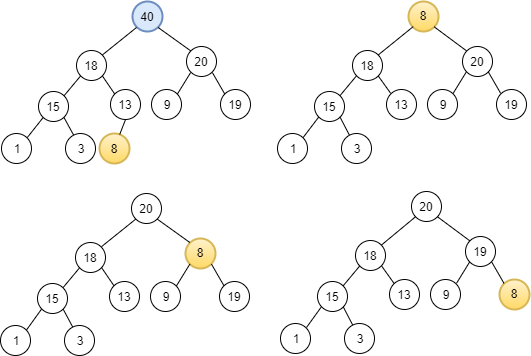
\includegraphics[width=.9\textwidth]{./image/cap3/heap-deletion}
    \end{center}
\end{frame}

%------------------------------
\subsection{Árboles binarios de búsqueda (BST)}

\begin{frame}{Árboles binarios de búsqueda (BST)}
    Un \blue{árbol binario de búsqueda} (\blue{binary search tree} o \blue{BST}) es un \redb{árbol binario} (no necesariamente completo) tal que el valor de cada nodo es $\geq$ que los de su subárbol izquierdo, y $\leq$ que los de su subárbol derecho.
    \begin{center}
        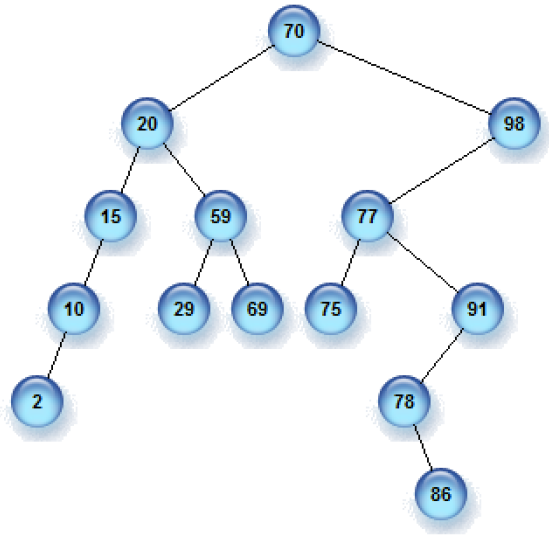
\includegraphics[width=.5\textwidth]{./image/cap3/BST}
    \end{center}
\end{frame}

\begin{frame}{Propiedades de un árbol binario de búsqueda}
    \begin{itemize}
        \item<1-> Un recorrido \redb{inorden} coincide con un orden de menor a mayor.
        \item<2-> El \blue{mínimo} es el primer nodo sin hijo izquierdo en un descenso por hijos izquierdos desde la raíz.
        \item<3-> El \blue{máximo} es el primer nodo sin hijo derecho en un descenso por hijos derechos desde la raíz.
    \end{itemize}
\end{frame}

\begin{frame}{Operaciones fundamentales}
    \begin{itemize}
        \item<1-> \blue{Buscar} un nodo
        \begin{enumerate}
            \item Se parte desde la raíz
            \item Se escoge el subárbol correspondiente respetando la relación $\leq$.
        \end{enumerate}
        \item<2-> \blue{Insertar} un nodo
        \begin{enumerate}
            \item Se busca el elemento en el árbol.
            \item Se inserta en el lugar donde debería haberse encontrado.\\[-1.5ex]
        \end{enumerate}
        \item<3-> \blue{Eliminar} un nodo\\[-1.5ex]
        \begin{enumerate}
            \item Si tiene 0 o 1 hijos, se elimina de manera natural.
            \item Si tiene 2 hijos, se intercambia por el máximo de su subárbol izquierdo (o por el mínimo de su subárbol derecho), y se elimina ese máximo (o ese mínimo).
        \end{enumerate}
    \end{itemize}
\end{frame}

\begin{frame}{Eliminación: Nodo con 0 hijos}
    \begin{center}
        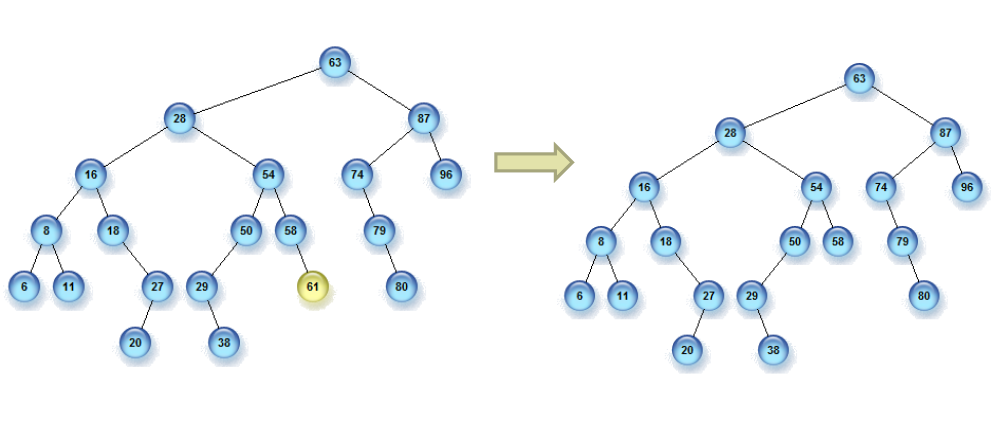
\includegraphics[width=\textwidth]{./image/cap3/BST-delete-0child}
    \end{center}
\end{frame}

\begin{frame}{Eliminación: Nodo con 1 hijo}
    \begin{center}
        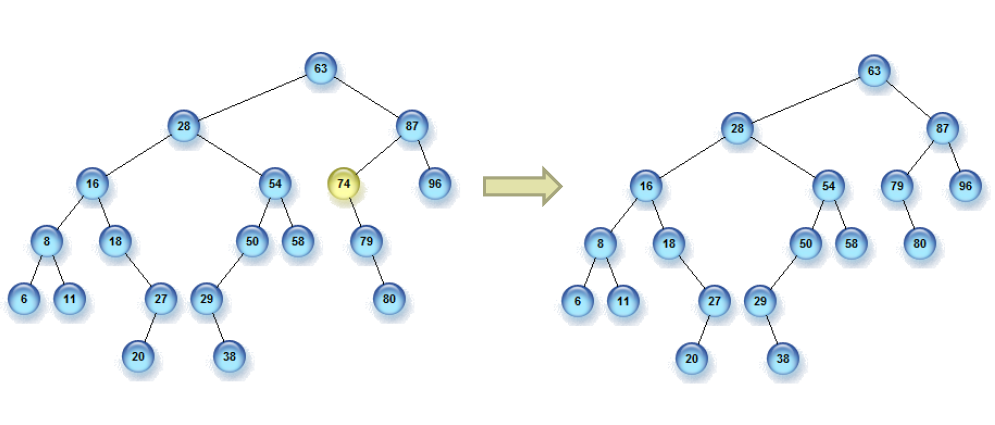
\includegraphics[width=\textwidth]{./image/cap3/BST-delete-1child}
    \end{center}
\end{frame}

\begin{frame}{Eliminación: Nodo con 2 hijos}
    \begin{center}
        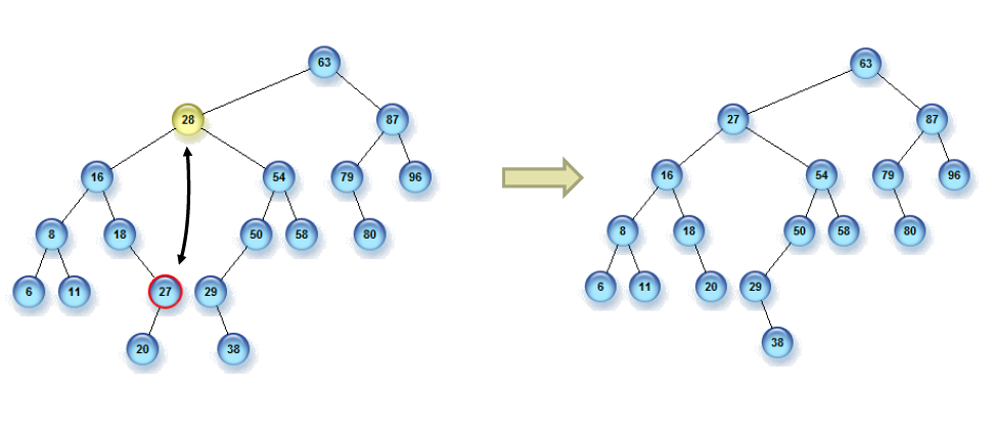
\includegraphics[width=\textwidth]{./image/cap3/BST-delete-2child}
    \end{center}
\end{frame}

%------------------------------
\subsection{Árboles balanceados o equilibrados}

\begin{frame}{Árboles balanceados}
    \begin{itemize}
        \item<1-> Un \blue{árbol balanceado} o \blue{equilibrado} es un \redb{árbol binario de búsqueda} restringido para que su altura sea logarítmica.
        \item<2-> Para mantener un árbol balanceado, se añaden instrucciones adicionales a las operaciones de inserción y borrado.
        \item<3-> Ejemplos:
        \begin{itemize}
            \item \blue{Árboles AVL}: la diferencia de altura entre subárboles izquierdo y derecho $\leq 1$.
            \item \blue{Árboles Rojo-Negro}
            \item \blue{Árboles biselados} (\blue{Splay trees})
        \end{itemize}
    \end{itemize}
\end{frame}

\begin{frame}{Arboles AVL}
  \begin{itemize}
\item Tipo de árbo inentado por Adelson-Valeskii-Landis (AVL).
\item Son arboles binarios donde todos sus elementos estan ordenados.
\end{itemize}
Sus principales características son:
\begin{itemize}
  \item Son equilibrados respecto a su altura, debido que las alturas de los sub árboles difieren a lo mas en 1.
  \item Factor de equilibrio: Sean AI y AD alturas de sub árbol izquierdo y derecho respectivamente se tiene que es equilibrado si {\mid AI-AD \mid \leq 1}.
\end{itemize}
\end{frame}

\begin{frame}{Estructura de nodo de arbol AVL. }
  NodoArbol\{ \\
    \quad \quad Objeto: dato;\\
    \quad \quad Hijo: izquierdo, derechos\\
    \quad \quad Integer: Factor de equilibrio;\\
  \}\\
  \begin{itemize}
    \item ¿Qué pasa si el FA no cumple la condicion 	\leq 1 ?
  \end{itemize}
\end{frame}

\begin{frame}{Rotación. }
\begin{itemize}
  \item II, ID, DD, DI
\end{itemize}
\end{frame}

\begin{frame}{Rotación Izquierda-Izquierda}
    \begin{center}
        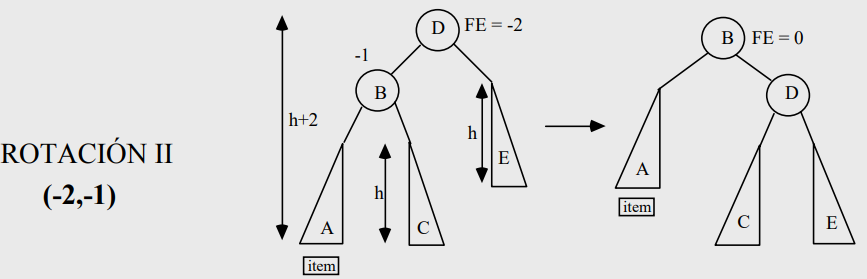
\includegraphics[width=\textwidth]{./image/cap3/II.PNG}
    \end{center}
\end{frame}
\begin{frame}{Rotación Derecha-Derecha}
    \begin{center}
        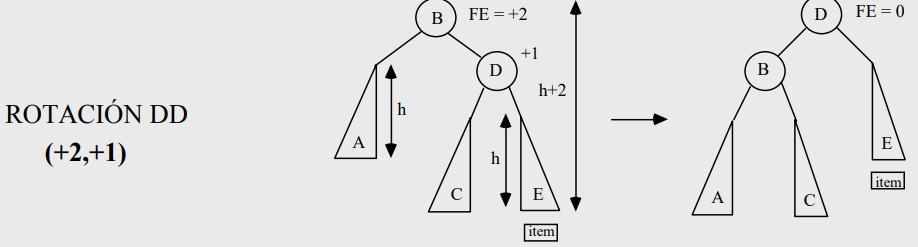
\includegraphics[width=\textwidth]{./image/cap3/DD.PNG}
    \end{center}
\end{frame}
\begin{frame}{Rotación Izquierda-Derecha}
    \begin{center}
        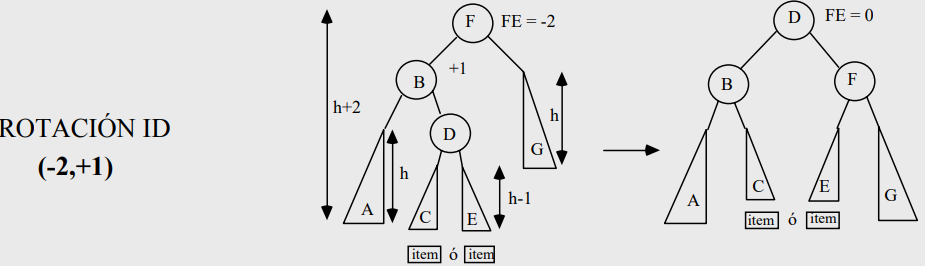
\includegraphics[width=\textwidth]{./image/cap3/ID.PNG}
    \end{center}
\end{frame}
\begin{frame}{Rotación Derecha-Izquierda}
    \begin{center}
        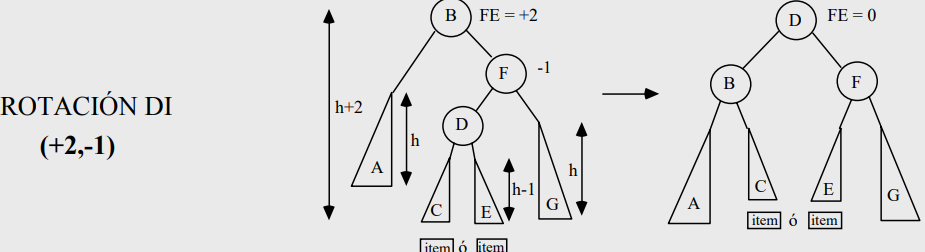
\includegraphics[width=\textwidth]{./image/cap3/DI.PNG}
    \end{center}
\end{frame}
\begin{frame}{Ejemplo:}
    \begin{center}
        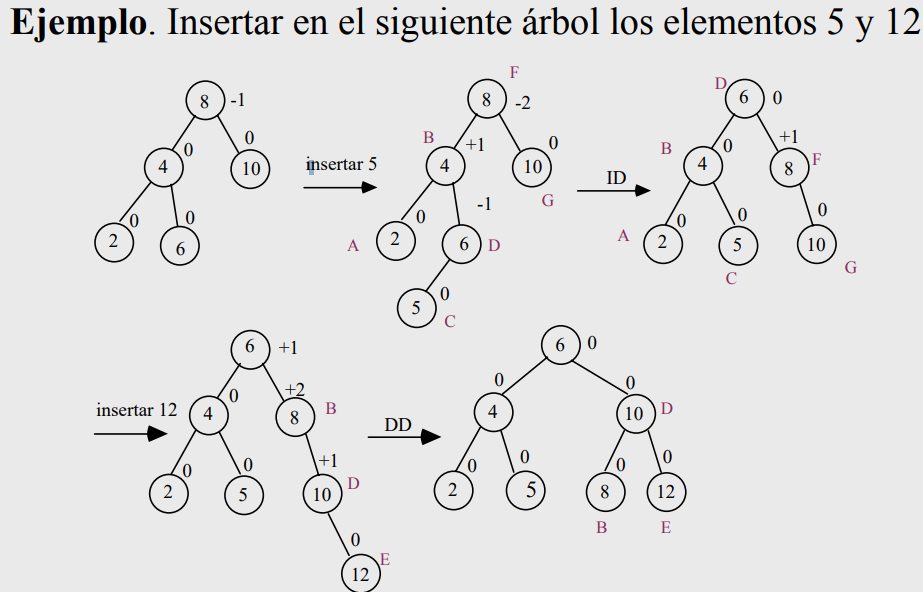
\includegraphics[width=\textwidth]{./image/cap3/avl_ej1.PNG}
    \end{center}
\end{frame}

%==============================
\section{Árboles B}

\subsection{Fundamentos}

\begin{frame}{Preliminares}
    \begin{itemize}
        \item<1-> Un \blue{árbol B} es una generalización de un árbol binario de búsqueda (BST) en que cada nodo puede tener \redb{$> 2$ hijos}.
        \item<2-> Es balanceado y de altura logarítmica, pero no binario, a diferencia de árboles AVL, Rojo-negro, biselados, etc.
        \item<3-> En cuanto a su complejidad computacional, en el ``peor caso'':
        \begin{tabular}{l|ccc}
                      & BST    & AVL         & B \\\hline
            Búsqueda  & $O(n)$ & $O(\log n)$ & $O(\log n)$\\
            Inserción & $O(n)$ & $O(\log n)$ & $O(\log n)$\\
            Borrado   & $O(n)$ & $O(\log n)$ & $O(\log n)$\\
        \end{tabular}\\[1.2ex]

        En el ``caso promedio'', todos son $O(\log n)$.
        \item<4-> A pesar de esto, el árbol B es una estructura de datos más eficiente para \redb{gandes volúmen de datos}, donde se requiere \redb{disminuir el número de accesos}: bases de datos, discos duros, memorias externas, sistemas de archivos.
    \end{itemize}
\end{frame}

\begin{frame}{Árboles-(a,b)}
    \begin{itemize}
        \item<1-> Un \blue{árbol-(a,b)} es un árbol de búsqueda balanceado, tal que:
        \begin{itemize}
            \item Si la raíz tiene hijos, su número está en el rango $[2,b]$.
            \item Los nodos internos tienen $[a,b]$ hijos, donde $2\leq a\leq \frac{b+1}{2}$.
            \item Todas las hojas están en el mismo nivel.
            \item Cada nodo con $k$ hijos tiene $k-1$ claves ordenadas ($\leq$):
            \begin{center}
            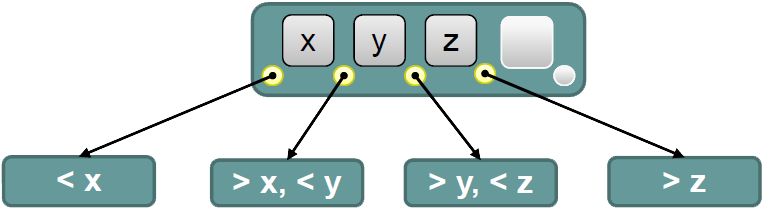
\includegraphics[width=.6\textwidth]{./image/cap3/(ab)-tree}
            \end{center}
        \end{itemize}
        \item<2-> Por ejemplo, en un \blue{árbol-(2,3)}:
        \begin{itemize}
            \item La raíz tiene 0, 2 o 3 hijos.
            \item Los nodos internos tienen 2 o 3 hijos.
        \end{itemize}
    \end{itemize}
\end{frame}

\begin{frame}{Árboles B}
    \begin{itemize}
        \item<1-> Un \blue{árbol B} \redb{de orden $m$} es un árbol-($d+1$, $2d+1$)\\con $m=2d+1$. Es decir:
        \begin{itemize}
            \item Si la raíz tiene hijos, su número está en el rango $[2,m]$.
            \item Los nodos internos tienen $[\lceil m/2\rceil,m]$ hijos.
            \item Todas las hojas están en el mismo nivel.
            \item Cada nodo con $k$ hijos tiene $k-1$ claves ordenadas ($\leq$):
        \end{itemize}
        \item<2-> Un árbol-B de orden 3 es un árbol-(2,3).
        \begin{center}
            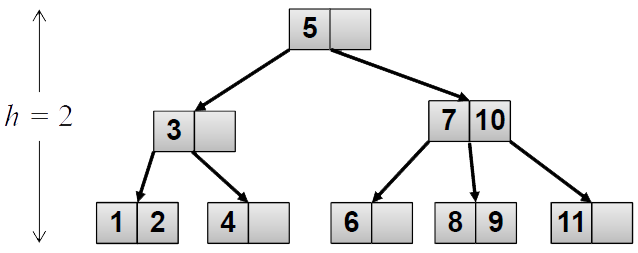
\includegraphics[width=.6\textwidth]{./image/cap3/(23)-tree}
        \end{center}
    \end{itemize}
\end{frame}

\subsection{Operaciones}

\begin{frame}{Reestructuraciones}
    \begin{center}
        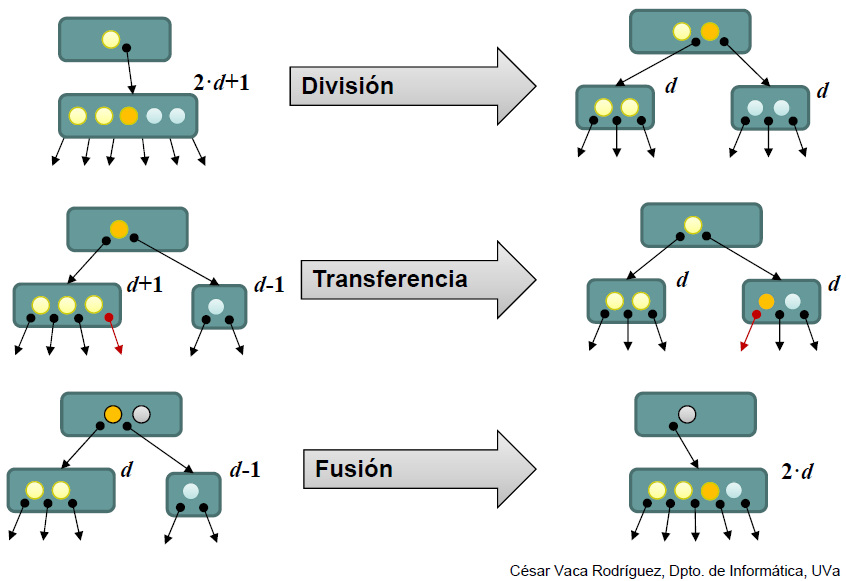
\includegraphics[width=.98\textwidth]{./image/cap3/b-tree-reestructurar}
    \end{center}
\end{frame}

\begin{frame}{Inserción - Sin reestructuración}
    \begin{itemize}
        \item Inserción del valor 2 en árbol B de orden 5 $\to$ árbol-(3,5)
    \end{itemize}
    \begin{center}
        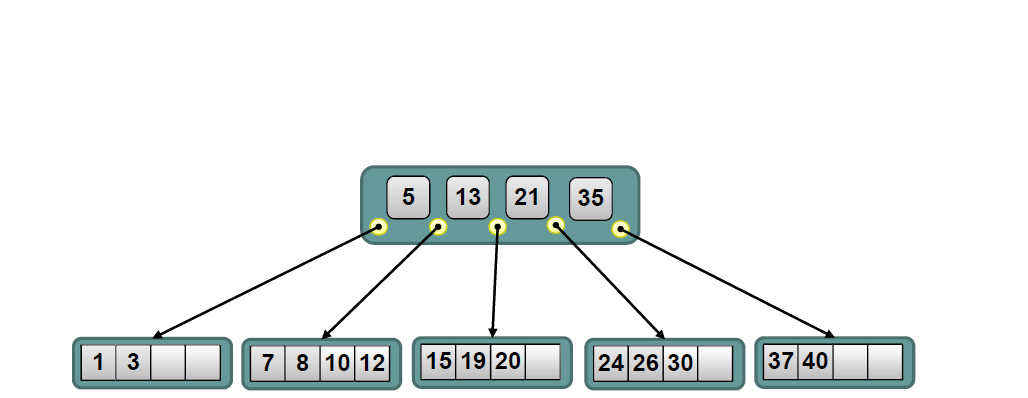
\includegraphics[width=\textwidth]{./image/cap3/b-tree-insert1}
    \end{center}
\end{frame}

\begin{frame}{Inserción - Sin reestructuración}
    \begin{itemize}
        \item Se busca el nodo hoja donde debe encontrarse el elemento
    \end{itemize}
    \begin{center}
        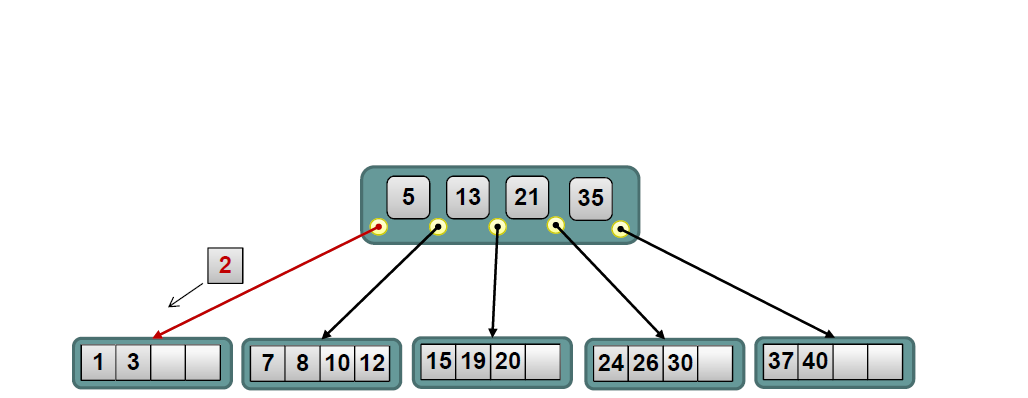
\includegraphics[width=\textwidth]{./image/cap3/b-tree-insert2}
    \end{center}
\end{frame}

\begin{frame}{Inserción - Sin reestructuración}
    \begin{itemize}
        \item Se inserta en orden en la hoja (desplazamiento). \redb{Fin}
    \end{itemize}
    \begin{center}
        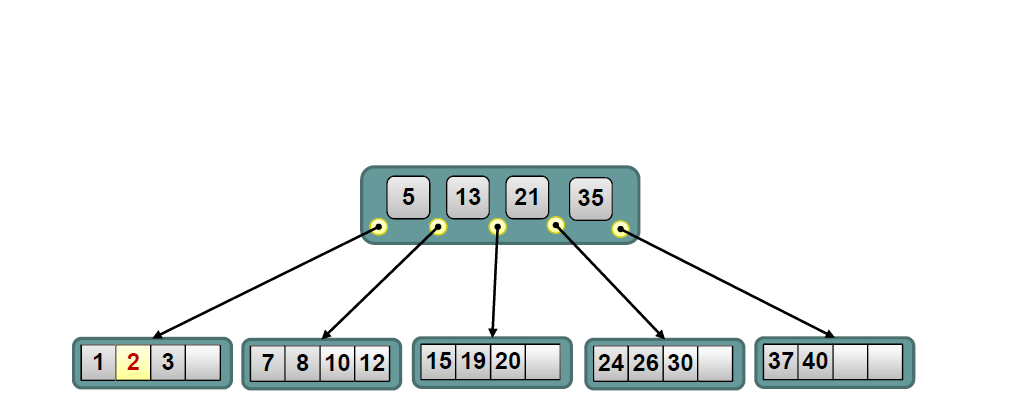
\includegraphics[width=\textwidth]{./image/cap3/b-tree-insert3}
    \end{center}
\end{frame}

\begin{frame}{Inserción - División de nodos}
    \begin{itemize}
        \item Inserción del valor 11
    \end{itemize}
    \begin{center}
        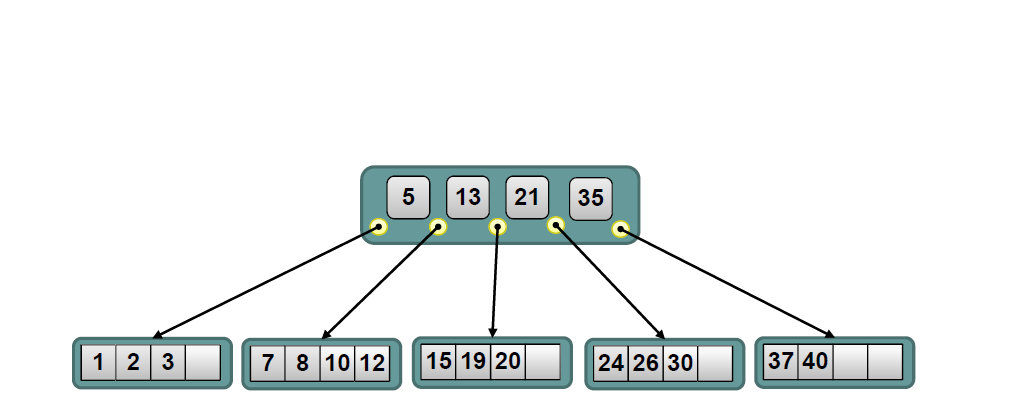
\includegraphics[width=\textwidth]{./image/cap3/b-tree-insert4}
    \end{center}
\end{frame}

\begin{frame}{Inserción - División de nodos}
    \begin{itemize}
        \item Se busca el nodo hoja donde debe encontrarse el elemento
    \end{itemize}
    \begin{center}
        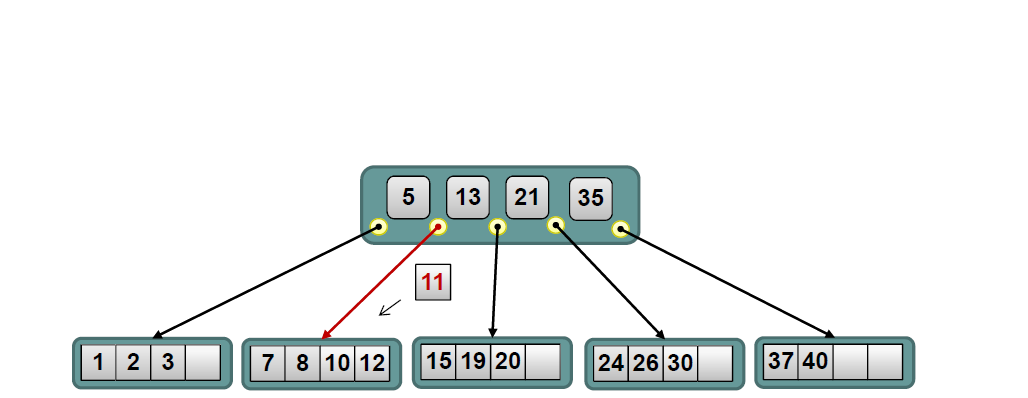
\includegraphics[width=\textwidth]{./image/cap3/b-tree-insert5}
    \end{center}
\end{frame}

\begin{frame}{Inserción - División de nodos}
    \begin{itemize}
        \item Se inserta en el nodo, pero sobrepasa el límite de claves (4)
    \end{itemize}
    \begin{center}
        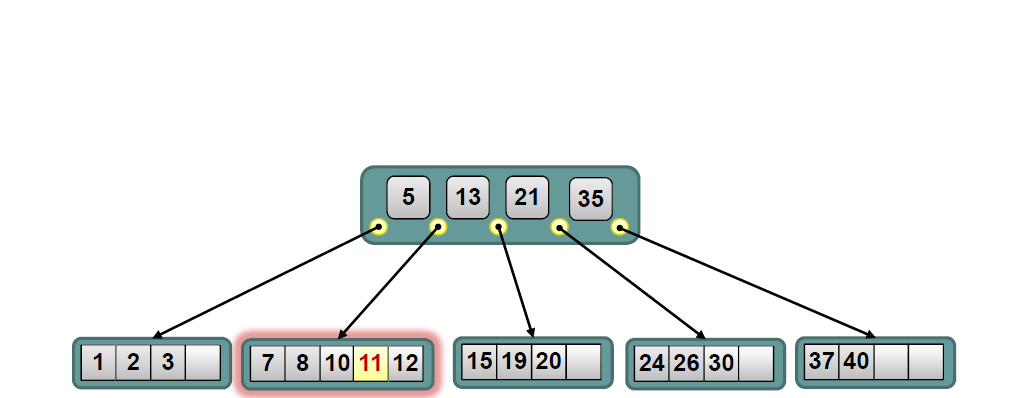
\includegraphics[width=\textwidth]{./image/cap3/b-tree-insert6}
    \end{center}
\end{frame}

\begin{frame}{Inserción - División de nodos}
    \begin{itemize}
        \item Se crea un nuevo nodo y se traslada la mitad derecha de los elementos a él.
        \item El elemento en posición media (10), junto con el enlace al nuevo nodo, se envía al padre para su inserción.
    \end{itemize}
    \vspace{-.2ex}

    \begin{center}
        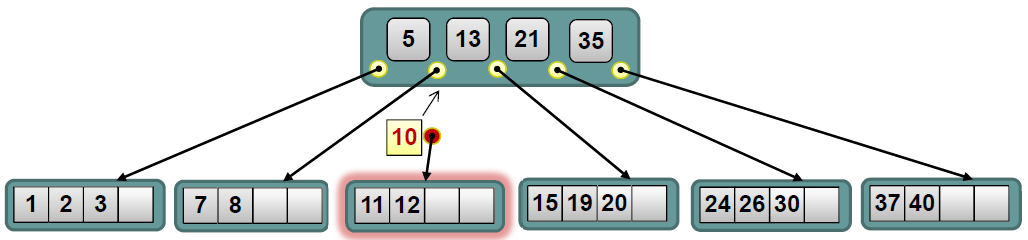
\includegraphics[width=\textwidth]{./image/cap3/b-tree-insert7}
    \end{center}
\end{frame}

\begin{frame}{Inserción - División de nodos}
    \begin{itemize}
        \item Se inserta en el padre, pero sobrepasa límite de claves (4).
    \end{itemize}
    \begin{center}
        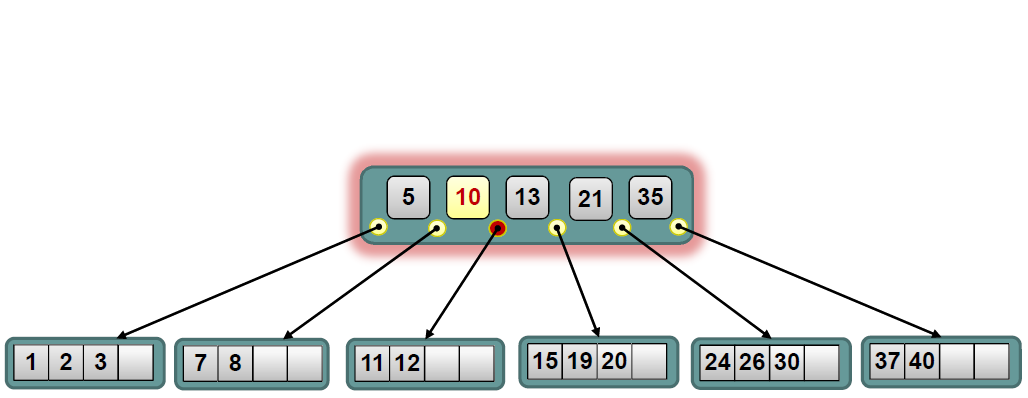
\includegraphics[width=\textwidth]{./image/cap3/b-tree-insert8}
    \end{center}
\end{frame}

\begin{frame}{Inserción - División de nodos}
    \begin{itemize}
        \item Se repite el proceso de división por la mitad.
    \end{itemize}
    \begin{center}
        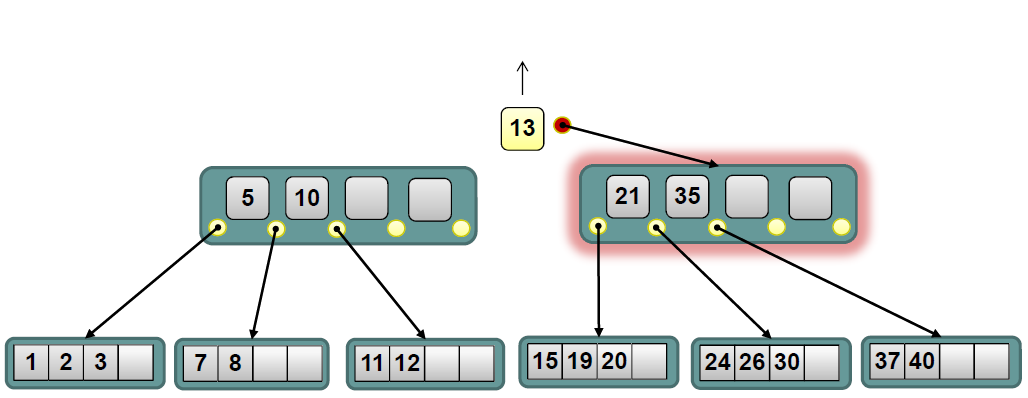
\includegraphics[width=\textwidth]{./image/cap3/b-tree-insert9}
    \end{center}
\end{frame}

\begin{frame}{Inserción - División de nodos}
    \begin{itemize}
        \item No hay padre $\to$ se crea nueva raíz con esa única clave. \redb{Fin}
    \end{itemize}
    \begin{center}
        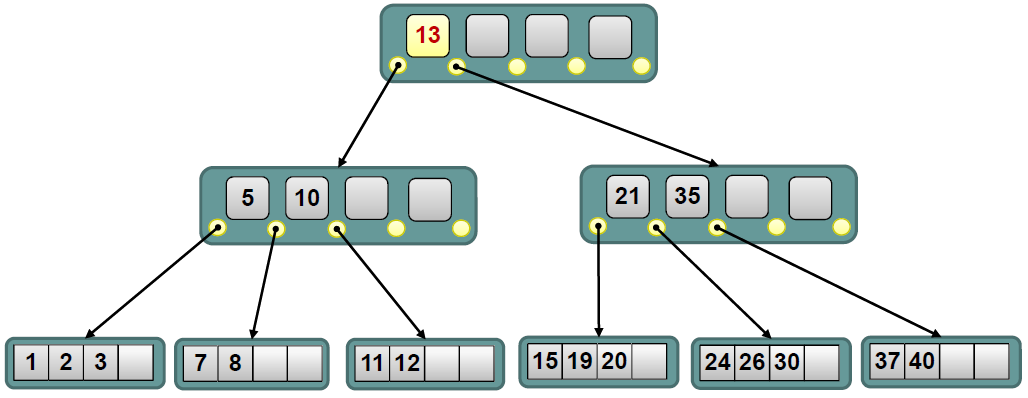
\includegraphics[width=\textwidth]{./image/cap3/b-tree-insert10}
    \end{center}
\end{frame}

\begin{frame}{Borrado - Sin estructuración}
    \begin{itemize}
        \item Borrado de clave 35. Se busca nodo donde está el elemento.
    \end{itemize}
    \begin{center}
        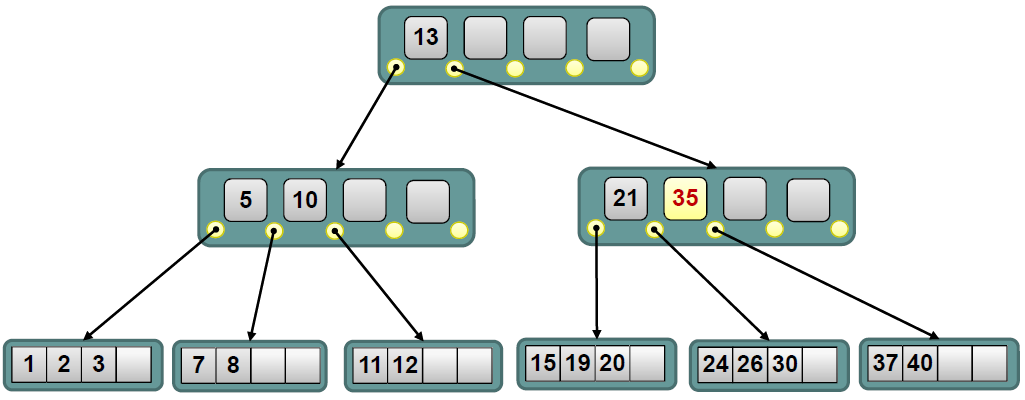
\includegraphics[width=\textwidth]{./image/cap3/b-tree-delete1}
    \end{center}
\end{frame}

\begin{frame}{Borrado - Sin estructuración}
    \begin{itemize}
        \item Es nodo interno: se intercambia con máx. de su hijo izquierdo
    \end{itemize}
    \begin{center}
        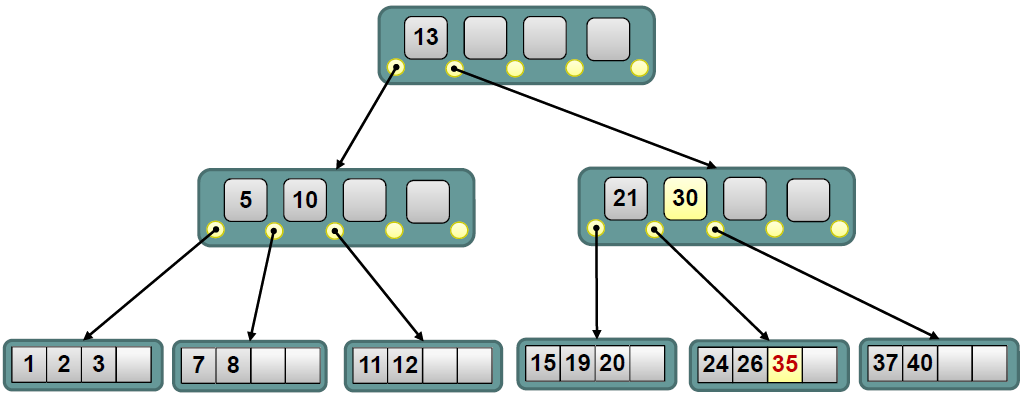
\includegraphics[width=\textwidth]{./image/cap3/b-tree-delete2}
    \end{center}
\end{frame}

\begin{frame}{Borrado - Sin estructuración}
    \begin{itemize}
        \item Se borra el elemento. \redb{Fin}
    \end{itemize}
    \begin{center}
        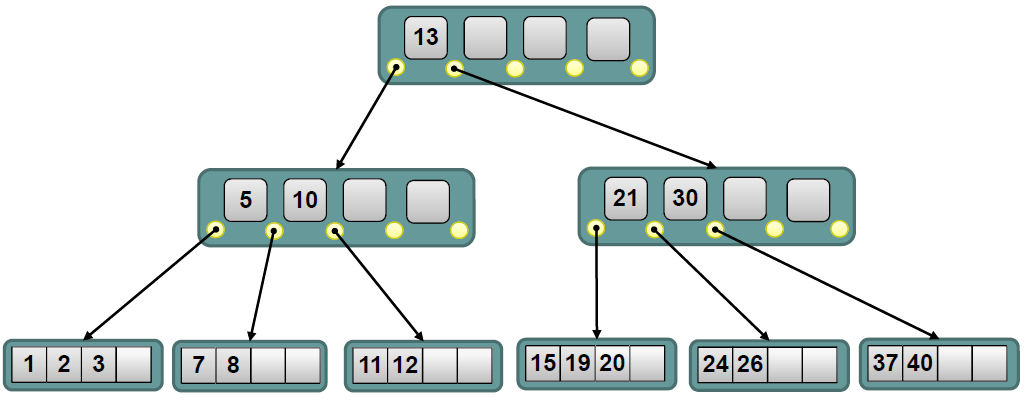
\includegraphics[width=\textwidth]{./image/cap3/b-tree-delete3}
    \end{center}
\end{frame}

\begin{frame}{Borrado - Transferencia}
    \begin{itemize}
        \item Borrado de la clave 8. Se busca el nodo.
    \end{itemize}
    \begin{center}
        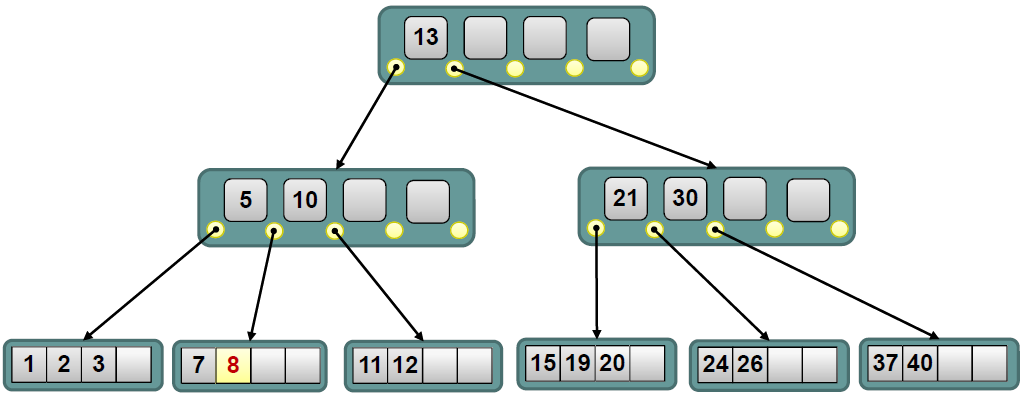
\includegraphics[width=\textwidth]{./image/cap3/b-tree-delete4}
    \end{center}
\end{frame}

\begin{frame}{Borrado - Transferencia}
    \begin{itemize}
        \item Se borra. Nodo queda con menos claves que permitidas (2).
    \end{itemize}
    \begin{center}
        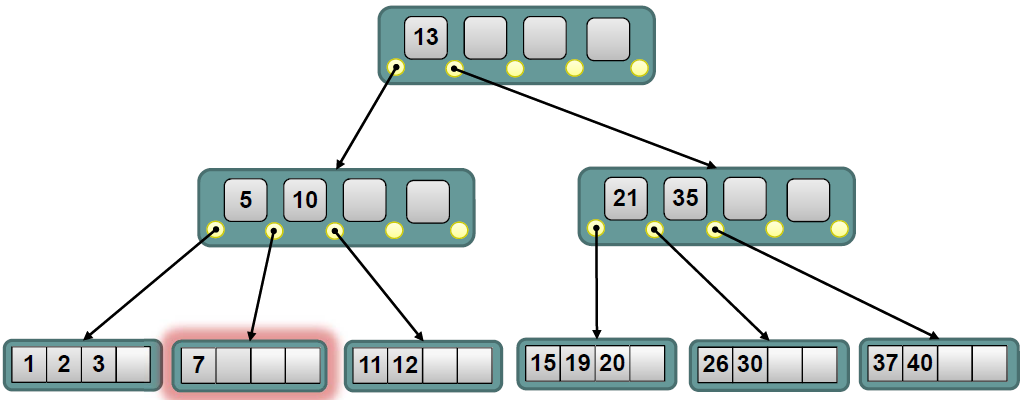
\includegraphics[width=\textwidth]{./image/cap3/b-tree-delete5}
    \end{center}
\end{frame}

\begin{frame}{Borrado - Transferencia}
    \begin{itemize}
        \item Se transfiere al padre la última clave del hermano más grande.
    \end{itemize}
    \begin{center}
        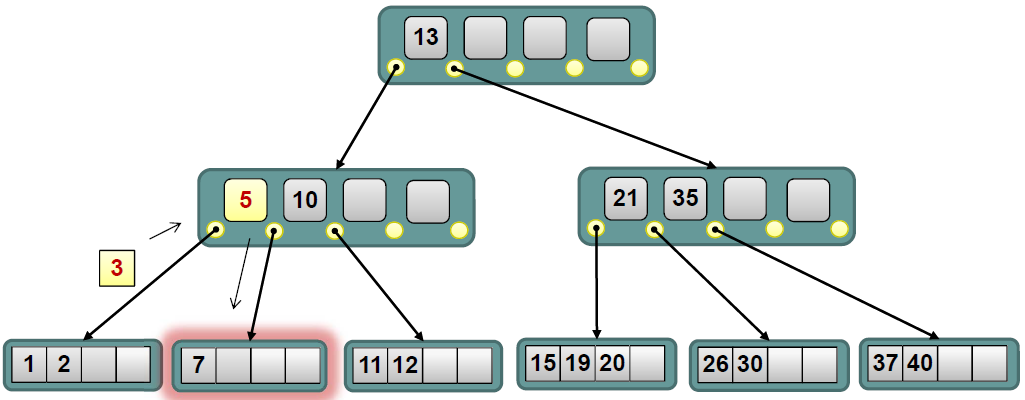
\includegraphics[width=\textwidth]{./image/cap3/b-tree-delete6}
    \end{center}
\end{frame}

\begin{frame}{Borrado - Transferencia}
    \begin{itemize}
        \item Se transfiere la antigua clave del padre al nodo. \redb{Fin}
    \end{itemize}
    \begin{center}
        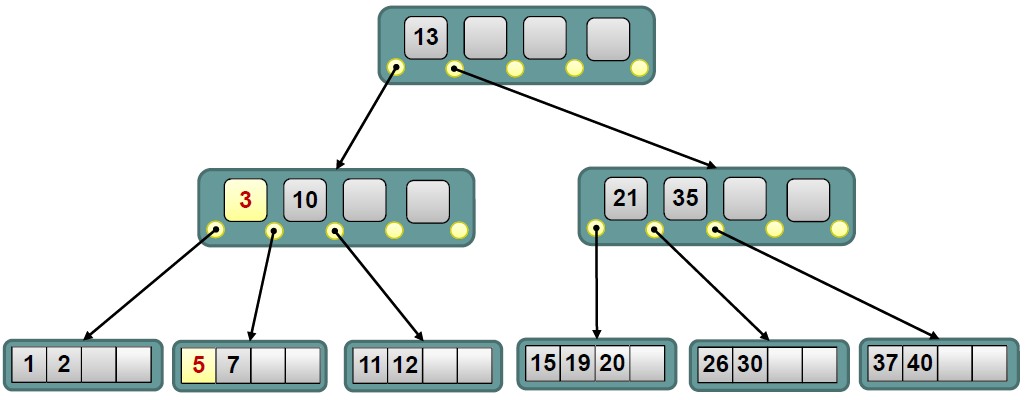
\includegraphics[width=\textwidth]{./image/cap3/b-tree-delete7}
    \end{center}
\end{frame}

\begin{frame}{Borrado - Fusión}
    \begin{itemize}
        \item Borrado de la clave 11. Se busca el nodo.
    \end{itemize}
    \begin{center}
        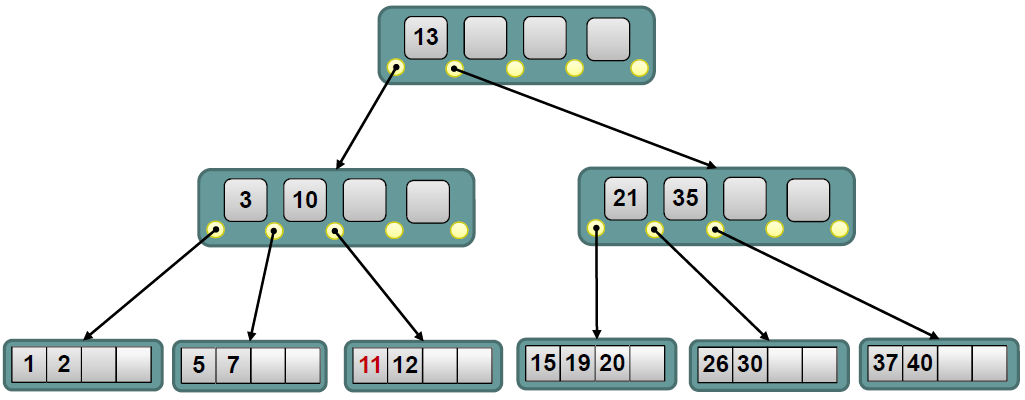
\includegraphics[width=\textwidth]{./image/cap3/b-tree-delete8}
    \end{center}
\end{frame}

\begin{frame}{Borrado - Fusión}
    \begin{itemize}
        \item Se borra. Nodo tiene 1 clave y su hermano no puede transferir.
    \end{itemize}
    \begin{center}
        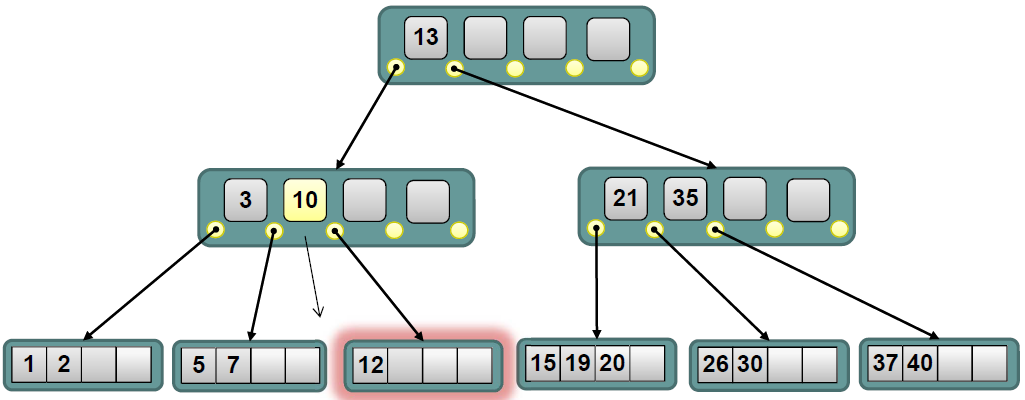
\includegraphics[width=\textwidth]{./image/cap3/b-tree-delete9}
    \end{center}
\end{frame}

\begin{frame}{Borrado - Fusión}
    \vspace{-2ex}

    {\small
    \begin{itemize}
        \item Hermanos se fusionan con clave del padre.\\[-1ex]
        \item Padre queda con 1 clave y su hermano no puede transferir.
    \end{itemize}}
    \vspace{-3ex}

    \begin{center}
        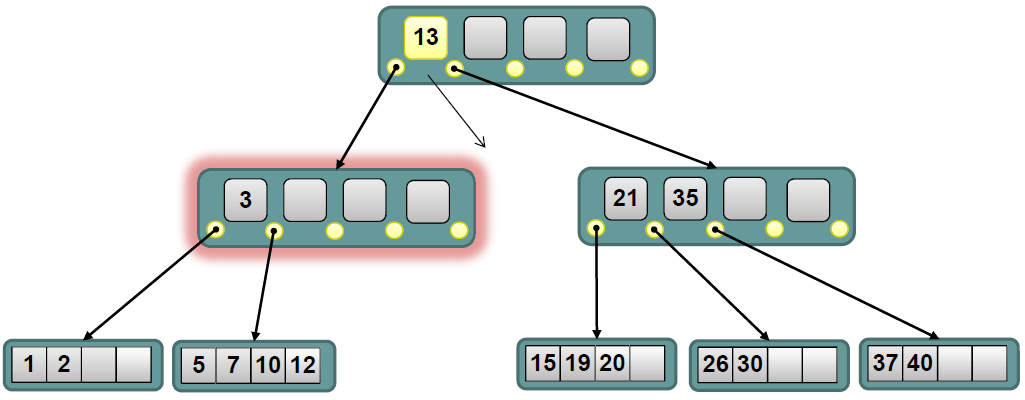
\includegraphics[width=\textwidth]{./image/cap3/b-tree-delete10}
    \end{center}
\end{frame}

\begin{frame}{Borrado - Fusión}
    \begin{itemize}
        \item Hermanos se fusionan con clave de raíz, que queda vacía.
    \end{itemize}
    \begin{center}
        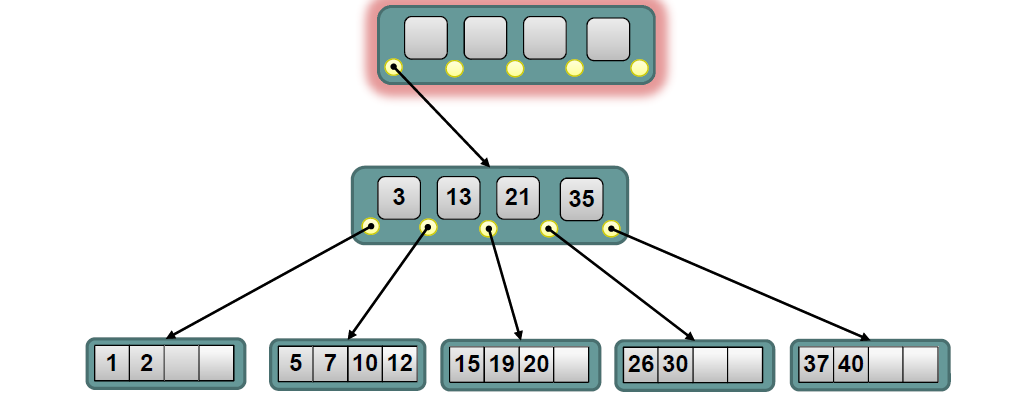
\includegraphics[width=\textwidth]{./image/cap3/b-tree-delete11}
    \end{center}
\end{frame}

\begin{frame}{Borrado - Fusión}
    \begin{itemize}
        \item Se elimina el nodo raíz. \redb{Fin}
    \end{itemize}
    \begin{center}
        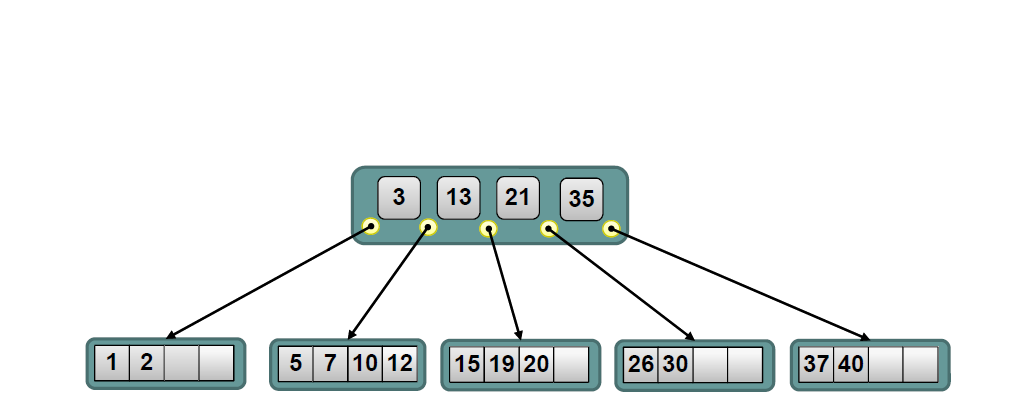
\includegraphics[width=\textwidth]{./image/cap3/b-tree-delete12}
    \end{center}
\end{frame}

\begin{frame}{Borrado - Fusión}
    \begin{itemize}
        \item Se elimina el nodo raíz. \redb{Fin}
    \end{itemize}
    \begin{center}
        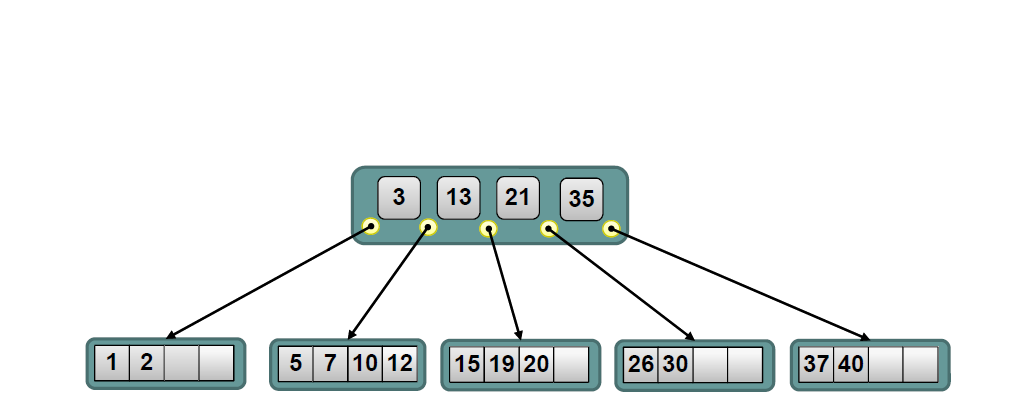
\includegraphics[width=\textwidth]{./image/cap3/b-tree-delete12}
    \end{center}
\end{frame}

\begin{frame}{Usos y variantes}
    \begin{itemize}
        \item<1-> Los árboles B y sus variantes se usan en:
        \begin{itemize}
            \item \redb{Gestores de bases de datos}
            \item \redb{Sistemas de archivos}: NTFS (Windows), HFS+ (Apple), btrfs, Ext4 (Linux)
        \end{itemize}
        \item<2-> Variantes principales:
        \begin{itemize}
            \item \blue{Árboles de prerecorrido}: Antes de insertar se realiza una búsqueda que divide todos los nodos llenos. El número máximo de claves es 2d+1.
            \item \blue{Árboles B+}: Sólo las hojas contienen elementos, los nodos internos contienen claves para dirigir la búsqueda (esas claves se encuentran también en los nodos hoja). Los nodos hoja forman una lista doblemente enlazada.
            \item \blue{Árboles B*}: El número mínimo de claves es 2/3 de la capacidad. Se fusionan 3 nodos en 2, y se dividen 2 nodos en 3.
        \end{itemize}
    \end{itemize}
\end{frame}

%------------------------------

\begin{frame}
 \begin{block}{Bibliografía recomendada}
  \begin{itemize}
    \item Weiss, M., Estructura de datos y algoritmos,\\ Addison-Wesley, 1995.
    \item Aho, Hopcroft y Ullman, Estructuras de datos y algoritmos, Addison-Wesley, 1988.
  \end{itemize}
 \end{block}
 \begin{block}{Recursos}
  \begin{itemize}
    \item Apuntes de César Vaca Rodríguez, Dpto. de Informática, Universidad de Valladolid, España, 11 Feb 2011.
    \item Wikimedia Commons.
    \item \url{http://www.cplusplus.com}
  \end{itemize}
 \end{block}
\end{frame}

\end{document}
